\documentclass[letterpaper,twoside,11pt,twocolumn]{article}

\usepackage{graphicx}
\usepackage{enumerate}
\graphicspath{ {./} }

\author{Elliot Hodge and Vella Karman\\\small{Central Arkansas Homeschool Academy}\small{\\2021-2022 Data Science Class}}
\date{December 31, 2021}
\title{\vspace{-2.2cm}Alone TV Show Data Regression}
\begin{document}
% generates the title
\maketitle

\noindent \textbf{Abstract} — In order to determine the correlation between the number of days contestants remained participating on the wilderness survival TV show ‘Alone’ and various other factors, we analyzed which tools from a set list of tools were brought and the average temperatures of the contest locations for each existing season of the show as of December 2021, excluding Season 4, which was treated as an outlier. The tools that were common to all participants were excluded from the analysis.

\section{Introduction}
\noindent The Alone TV show films competitors surviving the wilderness with a basic survival pack and ten items they choose from a list of approved gear. The regression analysis in the field of Data Science determined the correlation of average temperatures and the gear they selected to the number of days contestants survived the show. Data regression in Minitab showed the calculations for significance, correlation, and randomness, as well as a formula for the line of best fit. The researchers also used a set of random data to test the formula. The results are important for showing student comprehension of data regression and foundational concepts of data science and for potential Alone competitors.

The objective of this paper is to prove or disprove the hypothesis that a particular combination of tools will provide a measurable benefit to survival on Alone. The analysis included the number of days survived on Alone and the tools a competitor selected. The correlation between average hometown weather and average weather in the location of each season of Alone in September was also analyzed. 

This paper is structured as follows: Section 2 covers the experimental set-up and methodology, including why Season 4 was excluded. Section 3 presents the results of the analysis. Section 4 concludes the paper and shows the fitted line plot for the data. Section 5 includes the dataset before translation and the sources. 
\section{Experimental Setup and Methodology}
\subsection{Spreadsheet Creation}
\begin{enumerate}
    \item Using the list of gear each contestant took [1], a spreadsheet was created listing contestant first name, contestant last name.
    \item Using the aforementioned list [1], Season 4 contestants’ teammates’ first and last names were added to the spreadsheet. Other Seasons’ contestants, who did not work in teams, had ‘null’ listed for teammates’ first and last names.
    \item Using the aforementioned list [1], the season each contestant participated in was added to the spreadsheet. 
    \item Using the Wikipedia article on the Alone TV show [2], the days each contestant participated in the competition were added to the spreadsheet. Participants left because they opted out, the staff of Alone chose to medically evacuate them, or they won. In most seasons, the last person participating won, but in Season 7 any contestant who lasted 100 or more days won. 
    \item Using the Wikipedia article on the Alone TV show [2], whether the contestant was medically evacuated or not was added to the spreadsheet as a string value of Yes or No. 
    \item Using the Wikipedia article on the Alone TV show [2], the hometown for each contestant was taken, and a google search for average temperature was performed. The average temperature was added to the spreadsheet. If the average temperature was listed in an array of months, the month of September was used. 
    \item Using the Wikipedia article on the Alone TV show [2], the location for each season was taken, and a google search for the average temperature was performed. The average temperature was added to the spreadsheet. If the average temperature was listed in an array of months, the month of September was used. 
    \item For each allowed item on the list of allowed items [1], a column labeled with the item’s name was added to the spreadsheet. For each contestant or contestant pair, a string value of Yes was listed under the columns of the items each contestant selected, a string value of No was listed under the columns of the items the contestants did not select. If the contestant chose to take an item twice, Double was listed instead of Yes.
\end{enumerate}

The completed data set was uploaded to github [3].
\subsection{Minitab Setup}
\noindent Because Season 4 had two contestants working as a team, all rows from season four were removed as outliers. Because Season 4 was the only season in which multiple contestants were on a team together, the second contestant's first and last name columns were removed as they all contained the value ‘null’. 

Every item which no one brought, everyone brought, or only contestants from Season 4 brought was removed from the data set. Because of this, the Hatchet, Beef Jerky, Dried Snack Mix, Biltong, Hardtack Biscuits, Chocolate, Pemmican, Trail Mix, Flour, Salt, Rice/Sugar/Salt, Bear Canister, Bowl, Spoon, Lighter, Sleeping Pad, Sleeping Bag, Net Foraging Bag, Bar of Soap, Comb, Towel, Toothpaste, Floss, Shower Soap, and Razor columns were removed. 

The data was copied and pasted into MiniTab. Using the Fit Regression Model found in ‘Stat > Regression > Regression > Fit Regression Model,’ all items brought were added to the independent factors list. The average temperature in each contestant’s hometown and the average temperature in the contest location were added as independent variables as well. The days each contestant participated were added to the dependent variables list.

Using the equation generated, a prediction test was run, listing a number of items, an average home temperature, and an average contest location temperature. 

Using the same Fit Regression Model in a second test, this time only the average temperature data being added as independent variables, the days each contestant participated continued to be used as the dependent variable.

\section{Results}
\noindent With a 95\% confidence level, the analysis gave the results below for the correlation of tools chosen and tools not chosen with the days each contestant participated:

\noindent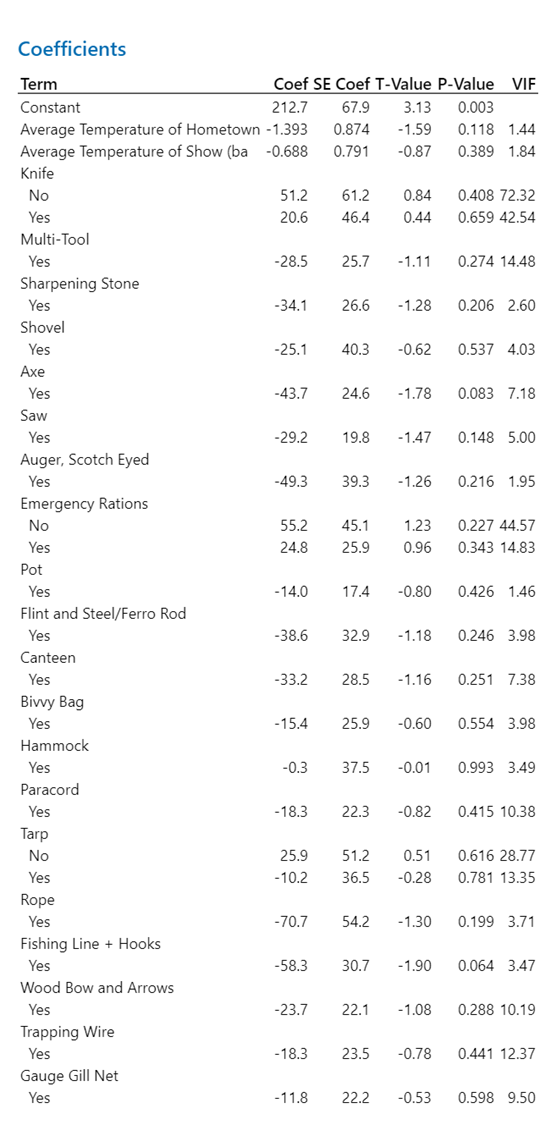
\includegraphics[width=0.5\textwidth]{./img1.png}

The p-value, showing statistical significance, ranged from 0.064 to 0.993 of the coefficient calculated for each item used as a variable. P-values above 0.5 are considered strong. The items which met that requirement and whether it was for or against bringing it were: Knife (Yes), Shovel (Yes), Bivvy Bag (Yes), Hammock (Yes), Tarp (Yes and No), and Gauge Gill Net (Yes). Only the Hammock shows a very strong (above 0.81) significance. 

The coefficient of determination (r²) was 35.42\% showing a low percentage of the data fits the line of best fit. This indicated a weak relationship. The residuals plot (below) had a random scatter of data, indicating random residuals.

\noindent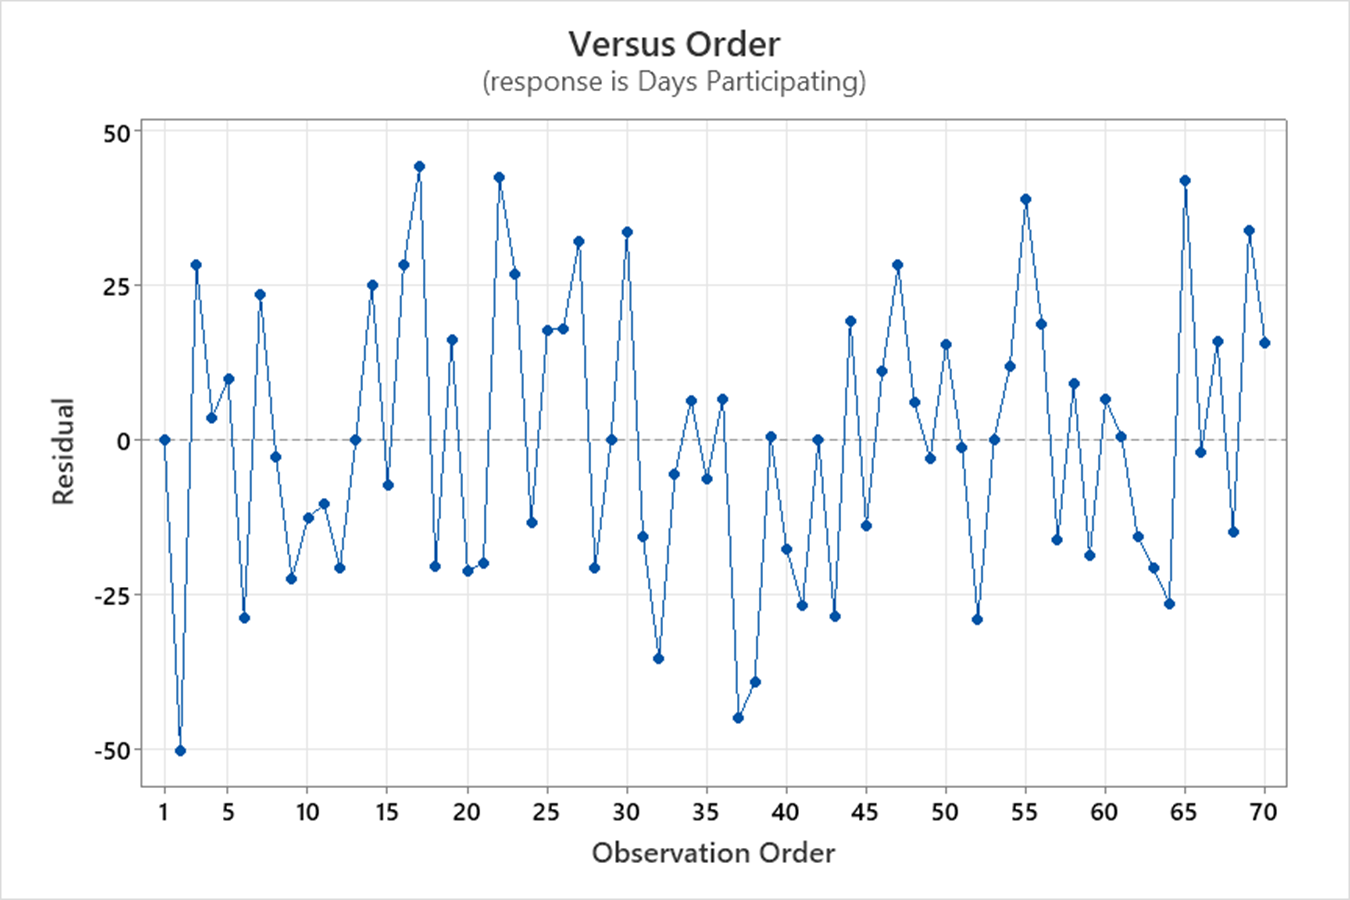
\includegraphics[width=0.5\textwidth]{./img2.png}

\noindent\textbf{Regression Equation}\\
The coefficient of determination demonstrated a weak relationship between the line of best fit and the data. While the p-values and coefficient of determination for the variables of the regression equation prove it to be inaccurate, a regression equation was still given. Due to the significance calculations and the relationship of the data to the line of best fit, we know this equation (below) cannot accurately predict results.

\noindent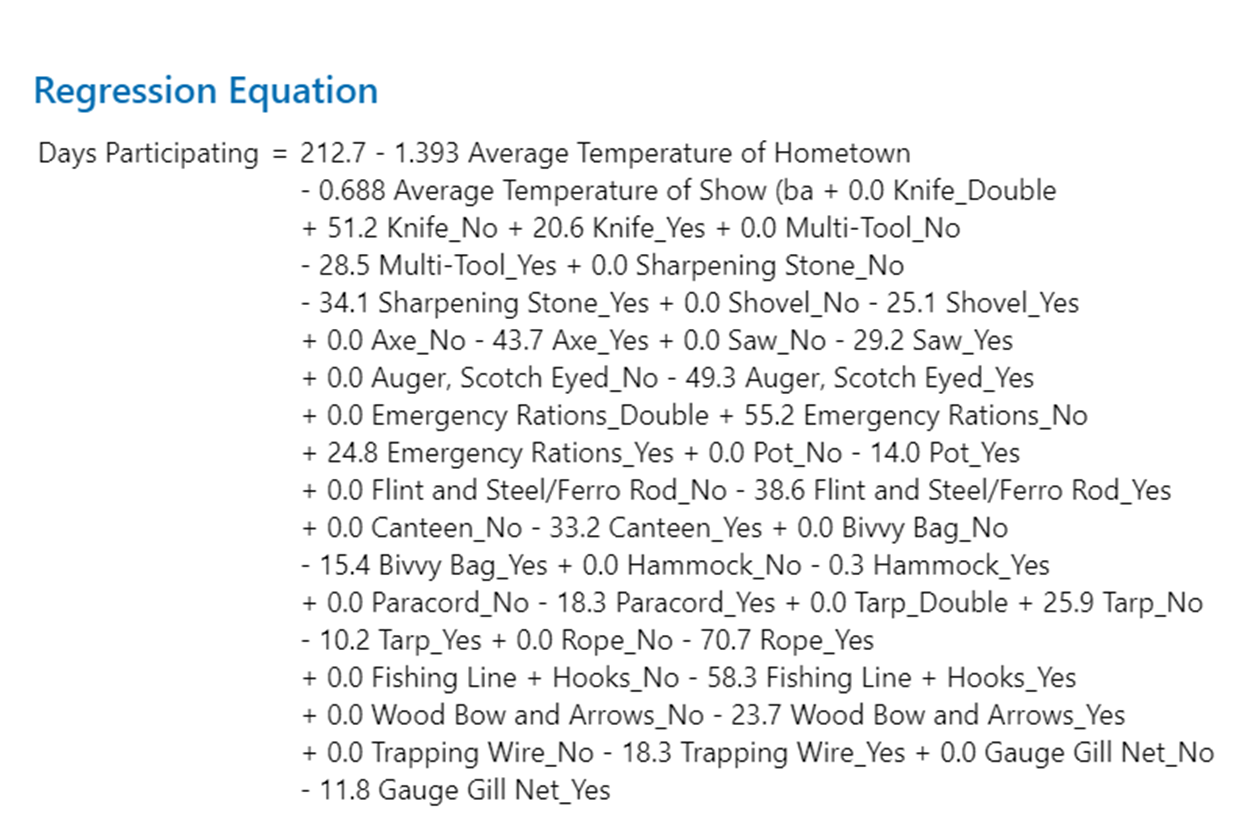
\includegraphics[width=0.5\textwidth]{./img3.png}

\noindent\textbf{Example Prediction}\\
The researchers entered random items into MiniTab to predict results using the regression equation. The settings are shown below.

\noindent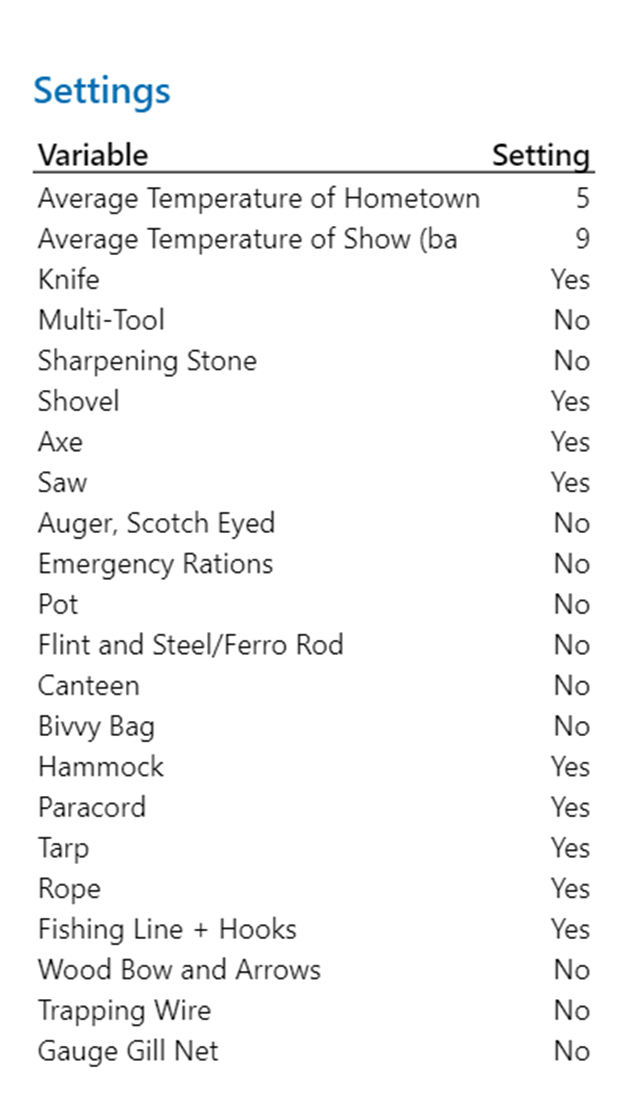
\includegraphics[width=0.5\textwidth]{./img4.png}

Minitab displayed a warning message for the PI point predicted, “XX denotes an extremely unusual point relative to predictor levels used to fit the model.” The predictions are below.

\noindent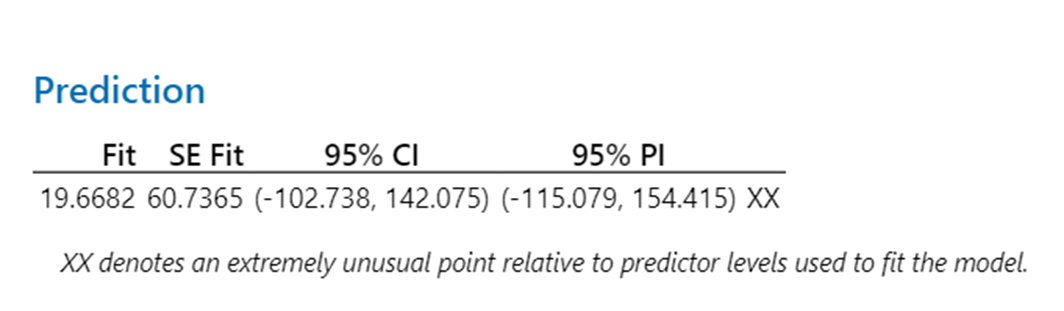
\includegraphics[width=0.5\textwidth]{./img5.png}

This prediction shows an unbelievably large range for the CI (confidence interval); from a negative number in the hundreds to a positive number in the hundreds. This indicated the margin of error is too high to be trusted. The PI value predicted demonstrates the inputs could be an outlier. Based on these two numbers, the fit (19.6682) cannot be trusted as an accurate prediction.

\noindent\textbf{Multiple Response Prediction}\\
The researchers set the computer to predict the inputs (temperature and gear) for the given output of the longest possible days based on the regression equation and the data available. The analysis is below.

\noindent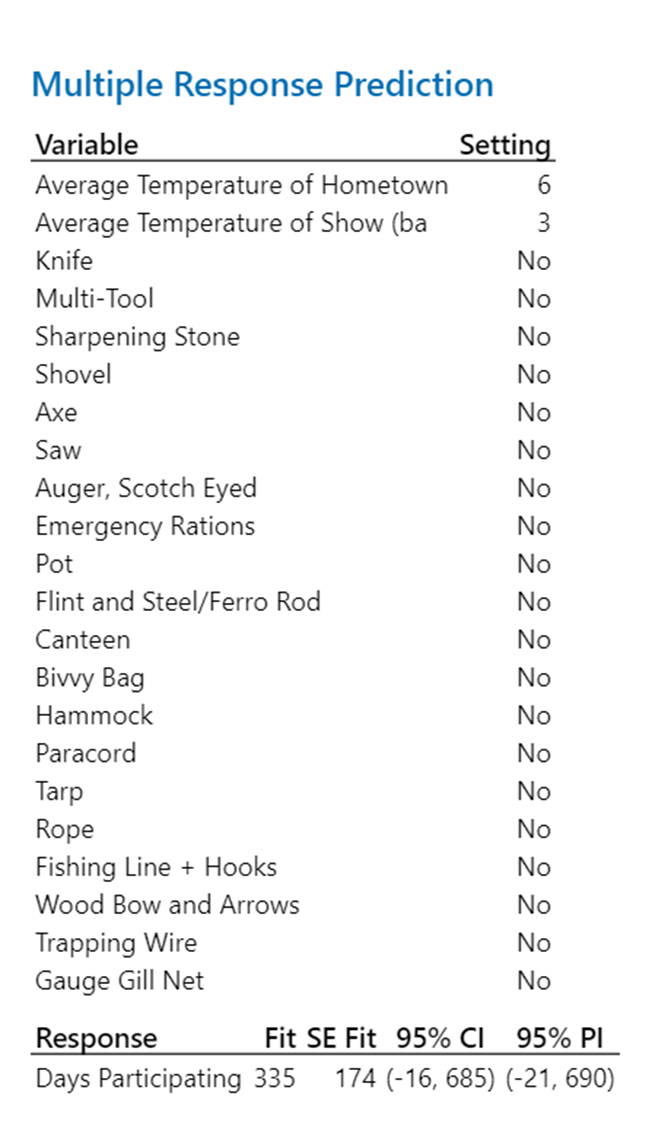
\includegraphics[width=0.4\textwidth]{./img6.png}

According to this prediction, the best way to succeed would be to bring no items at all.\\

\noindent\textbf{Temperature}\\
The other factor analyzed was the average hometown temperature in the same month as the season was filmed compared to the average temperature at the location of filming. The fitted line plot for this analysis (below) has an r² value of 8.9\% which indicates the line of best fit explains that percentage of the data. No correlation was found. 

\noindent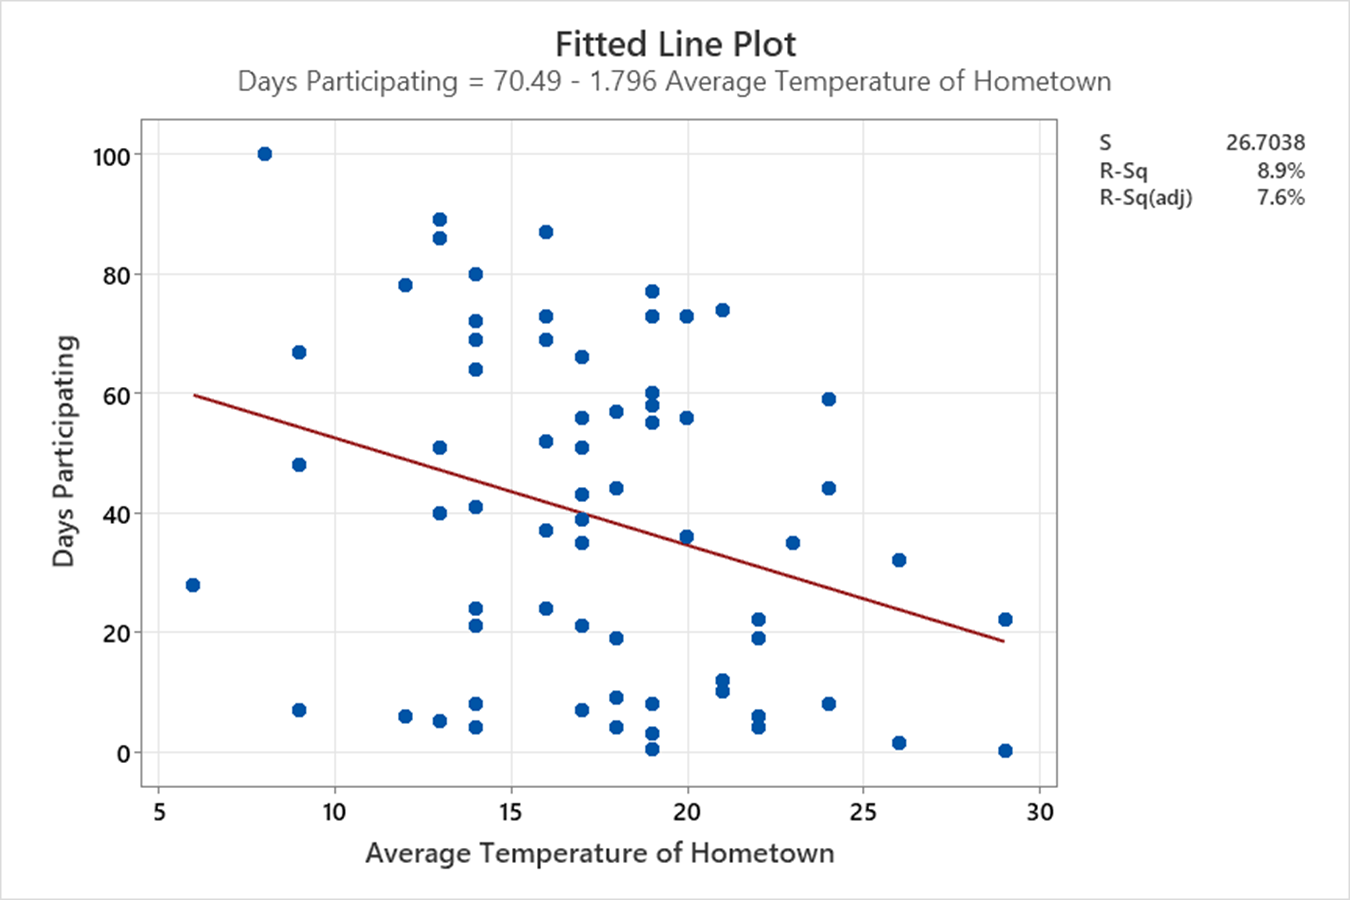
\includegraphics[width=0.5\textwidth]{./img7.png}

The equation given was Days Participating + 70.49 - 1.796 Average Temperature of Hometown. The data indicates this equation can not accurately predict results either. 

\section{Conclusion}

Based on the data analysis, the hypothesis that a particular combination of tools will provide a measurable benefit to survival on Alone must be rejected.

The analysis showed no correlation between tools a competitor decided to bring and the number of days they lasted. It is possible the skill set of the competitor is the defining factor, but more research would have to be done to reach a conclusion. 

The analysis showed no correlation between the average hometown temperature in September and the average temperature where the season was shot.

There is no relevant further research to do on this topic. 

\section{References}

\begin{enumerate}[ {[}1{]} ]
    \item Bushcraft Info. Alone Prohibited Items\\ \& Gear List.  https://bushcraftinfo.com/alone-prohibited-items-gear-list/. 
    \item Wikipedia. Alone (TV series). Online encyclopedia: https://en.wikipedia.org/wiki/\\Alone\_(TV\_series), 2015. revision 16:48, December 17th 2021.
    \item Github. Alone Dataset. https://github.\\com/Craftidore/Assignments/blob/main/20\\21-22/Data\%20Science/Alone\%20Dataset.csv. 
\end{enumerate}
\end{document}